\thispagestyle{empty}

\begin{center}
    {\LARGE\bf Abstract}
\end{center}

%Include an abstract for your project. This should be no more than 300 words.
Sir John ``Kyffin'' Williams was a landscape painter from Wales whose work was predominantly based 
in Wales and Patagonia. He studied at the Slade, one of Britain's top art schools, after epilepsy
ended his career in the army during the second world war. This epilepsy made Kyffin Williams 
sensitive to light and is the reason his work gets darker over time\cite{Harris2011How}.

Gareth Lloyd Roderick, a PhD student in the National Library of Wales, has
collected data such as the date or location, of these paintings. This data allows for some 
interesting analysis; particularly that of temporal or geographical classification of a given 
painting. That is being able to take a painting and decide the year or location in which it was
painted from a database of existing, known, works by Kyffin Williams.

Temporal analysis will be the focus of this project as it allows for a diverse range of techniques;
from statistical analysis of colour values of the paintings to looking at the length and style of 
paintbrush strokes. Geographical analysis would likely be very difficult, especially as the locations
depicted were often sketched on-site then painted in a studio.

Whilst it would be nice to be able to predict the age of a painting with no known year, it is far
more interesting to try to guess the year of paintings for which the date is known. This project 
will use leave-one-out cross-validation to help measure the effectiveness and validity of the 
analysis techniques employed in this project. Leave-one-out validation can be used with this 
project as the data set is small enough not to incur large performance overheads and the overall
speed of the program is irrelevant so long as it completes within a decent amount of time.

One major limitation with this is it also includes the technique used for classification, some
techniques might work better with K-Nearest Neighbour whilst other might benefit from more complex
methods of classification. This means I will either have to stick with a single classification
algorithm and hope it's a good one for all techniques. Or I could find the best machine learning
technique for each individual analysis technique, then perform comparison. This does assume that
the best machine learning technique for every analysis technique exists within the scope of the
project.

As there has been a lot of research into this topic there is an introductory paper to the 
literature\cite{Stork2009Computer}, this paper specifies a lot of useful papers, including papers
like the \textsc{authentic} project\cite{Berezhnoy2005Authentic}.
%TODO Key Papers

Some examples of Kyffin Williams' work show the changes in his style over time; his early work as
shown in figure~\ref{fig:kyffin-early} often contained a lot of strokes and quite a lot of bright
colour. Comparing it to the work in around the middle of his career show in figure~\ref{fig:kyffin-mid}, there are visible differences;
the colours used are a lot darker and the strokes on the canvas are a lot more confident, leading
to a more ``blocky'' feel. His later work, shown in figure~\ref{fig:kyffin-late} retains this 
``blocky'' feel and the darker colours, but has a lot more detail like some of the paintings from
his earlier period.

There is also a period in 1969 where Kyffin Williams visited Patagonia and did quite a few works
in that area; these are visually very distinct as they use a lot of orange colours not common to
Welsh landscapes. Some of this work is shown in figure~\ref{fig:kyffin-patagonia}.

\begin{figure}[h]
\centering
\begin{subfigure}[b]{0.4\textwidth}
  \centering
  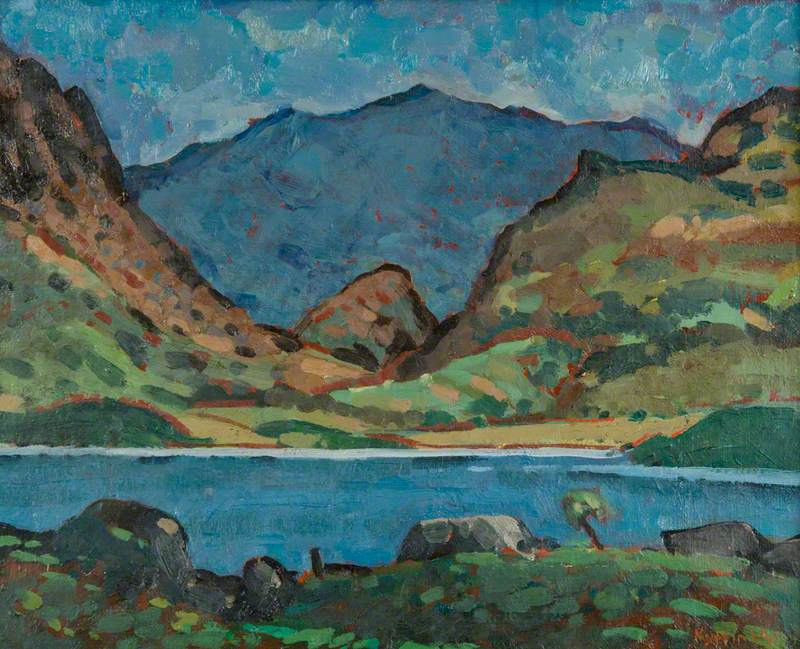
\includegraphics[width=\textwidth]{img/acnmw_acnmw_da006778_02_large.jpg}
  \caption{Snowdon from Llyn Nantle (1945)}
\end{subfigure}
\begin{subfigure}[b]{0.4\textwidth}
  \centering
  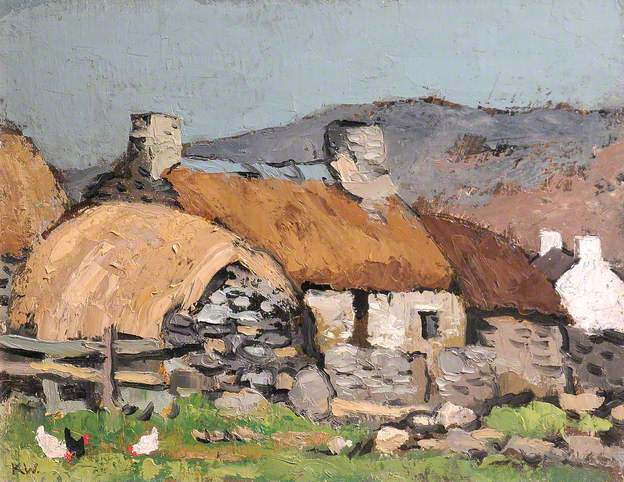
\includegraphics[width=\textwidth]{img/nwm_oym_1_90_624x544.jpg}
  \caption{Swtan (1947)}
\end{subfigure}
\caption{Early works by Kyffin Williams}
\label{fig:kyffin-early}
\end{figure}

\begin{figure}[h]
\centering
\begin{subfigure}[b]{0.4\textwidth}
  \centering
  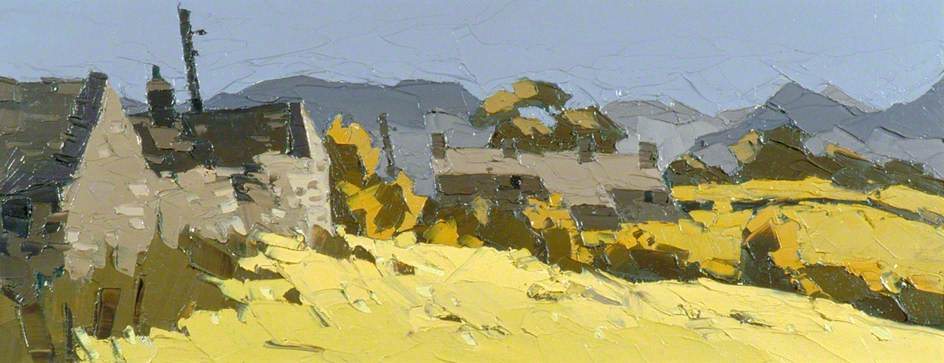
\includegraphics[width=\textwidth]{img/gac_gac_13839_large.jpg}
  \caption{Nant Ffrancon from Llandegfan (1970)}
\end{subfigure}
\begin{subfigure}[b]{0.4\textwidth}
  \centering
  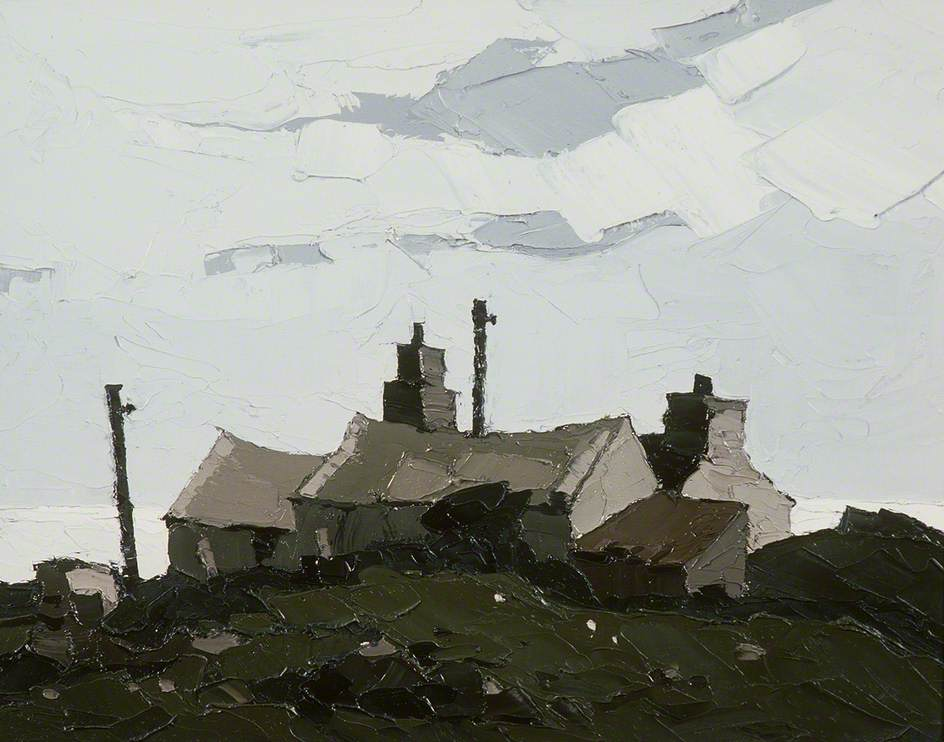
\includegraphics[width=\textwidth]{img/nlw_nlw_gcf02283_large.jpg}
  \caption{Farm, Llanfairynghornwy (1974)}
\end{subfigure}
\caption{Works by Kyffin Williams in the middle of his career}
\label{fig:kyffin-mid}
\end{figure}

\begin{figure}[h]
\centering
\begin{subfigure}[b]{0.4\textwidth}
  \centering
  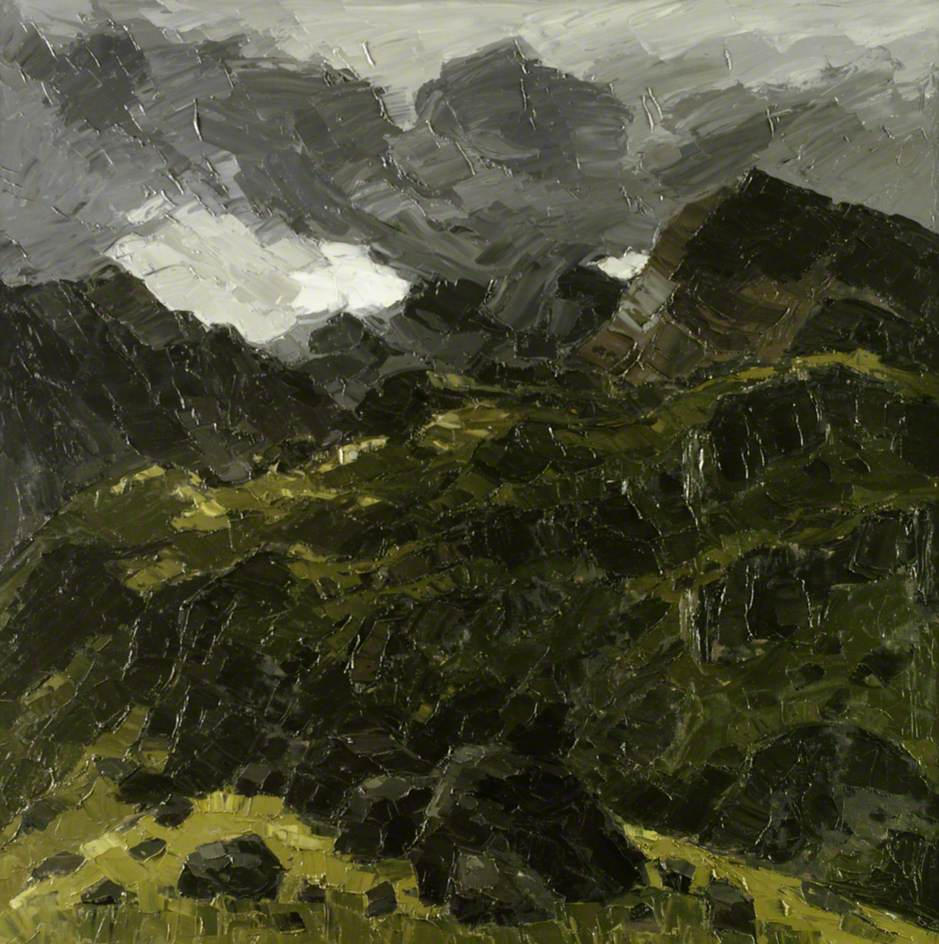
\includegraphics[width=\textwidth]{img/nlw_nlw_gcf06690_large.jpg}
  \caption{Pengwyryd (1999)}
\end{subfigure}
\begin{subfigure}[b]{0.4\textwidth}
  \centering
  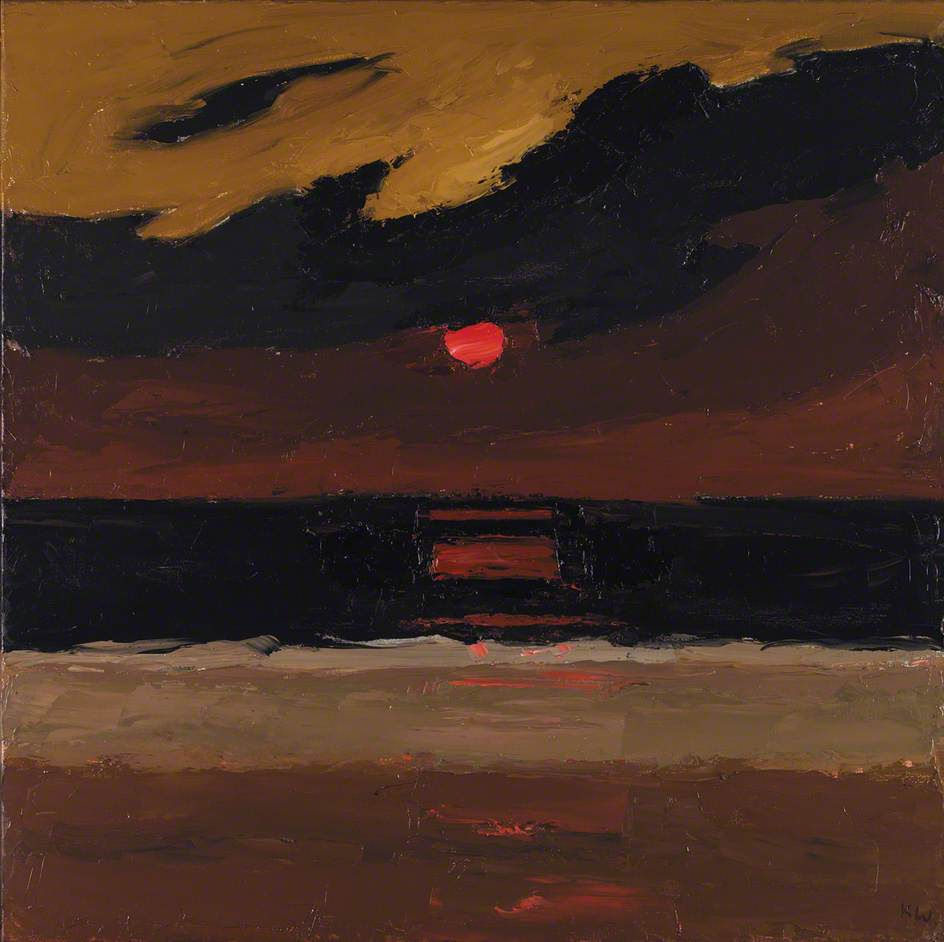
\includegraphics[width=\textwidth]{img/nlw_nlw_gcf08104_large.jpg}
  \caption{Sunset, Anglesey (2004)}
\end{subfigure}
\caption{Works by Kyffin Williams towards the end of his career}
\label{fig:kyffin-late}
\end{figure}

\begin{figure}[h]
\centering
\begin{subfigure}[b]{0.4\textwidth}
  \centering
  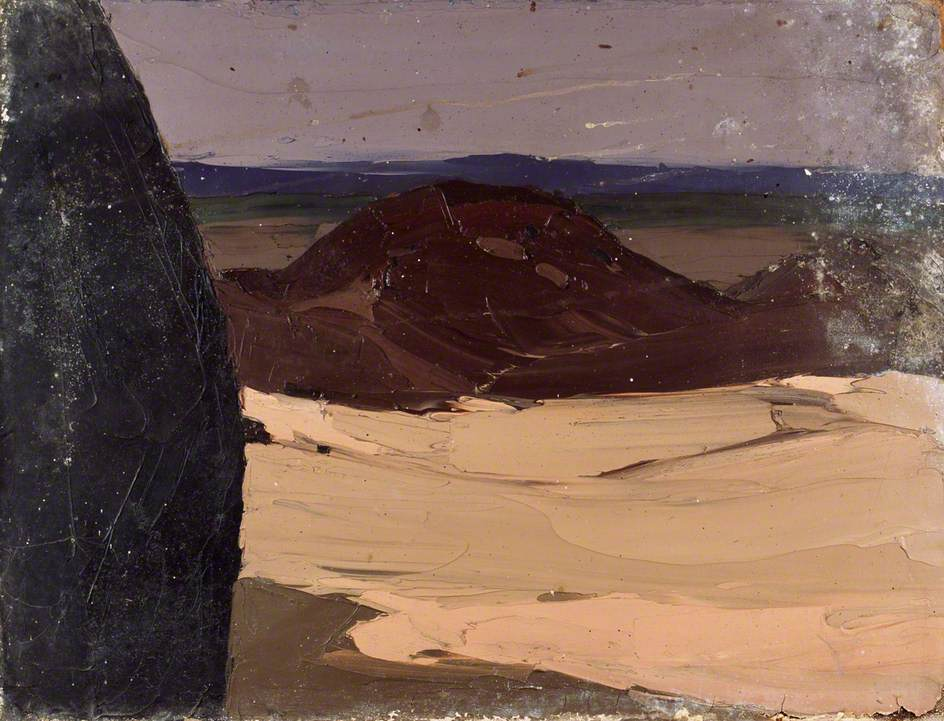
\includegraphics[width=\textwidth]{img/nlw_nlw_kwf00325_large.jpg}
  \caption{Paith, Patagonia (1969)}
\end{subfigure}
\begin{subfigure}[b]{0.4\textwidth}
  \centering
  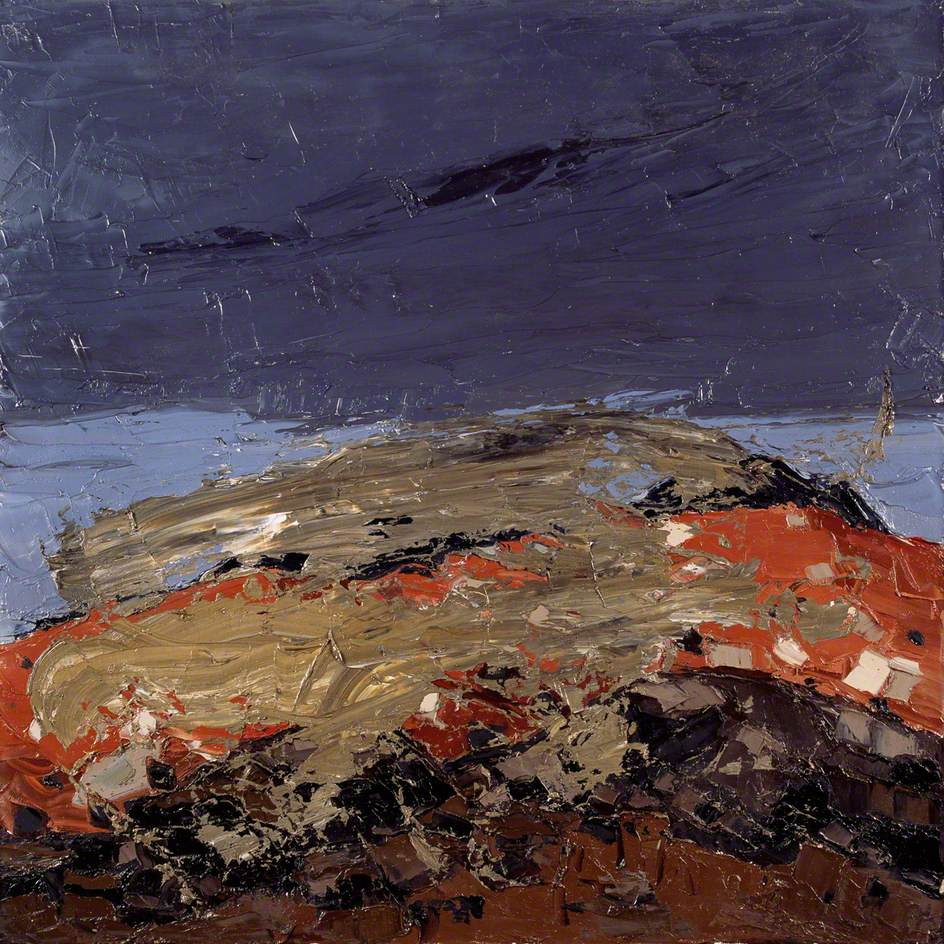
\includegraphics[width=\textwidth]{img/nlw_nlw_kwf00103_large.jpg}
  \caption{Patagonian Landscape (1969)}
\end{subfigure}
\caption{Works by Kyffin Williams from his trip to Patagonia}
\label{fig:kyffin-patagonia}
\end{figure}

At current I have had one meeting with both Lloyd and Hannah to discuss the current progress of 
the project and where we see the project progressing to. Lloyd was impressed by the current state
of the project and was looking forward to see where it was leading to.

We also discussed the potential of getting a paper published out of this project.
